% Judul dokumen
\title{Buku Tugas Akhir ITS}
\author{Musk, Elon Reeve}

% Pengaturan ukuran teks dan bentuk halaman dua sisi
\documentclass[12pt,twoside]{report}

% Pengaturan ukuran halaman dan margin
\usepackage[a4paper,top=30mm,left=30mm,right=20mm,bottom=25mm]{geometry}

% Pengaturan ukuran spasi
\usepackage[singlespacing]{setspace}

% Pengaturan detail pada file PDF
\usepackage[pdfauthor={\@author},bookmarksnumbered,pdfborder={0 0 0}]{hyperref}

% Pengaturan jenis karakter
\usepackage[utf8]{inputenc}

% Pengaturan pewarnaan
\usepackage[table,xcdraw]{xcolor}

% Pengaturan kutipan artikel
\usepackage[style=apa, backend=biber]{biblatex}

% Package lainnya
\usepackage{changepage}
\usepackage{enumitem}
\usepackage{eso-pic}
\usepackage{txfonts} % Font times
\usepackage{etoolbox}
\usepackage{graphicx}
\usepackage{lipsum}
\usepackage{longtable}
\usepackage{tabularx}
\usepackage{wrapfig}
\usepackage{float}

% Definisi untuk "Hati ini sengaja dikosongkan"
\patchcmd{\cleardoublepage}{\hbox{}}{
  \thispagestyle{empty}
  \vspace*{\fill}
  \begin{center}\textit{[Halaman ini sengaja dikosongkan]}\end{center}
  \vfill}{}{}

% Pengaturan penomoran halaman
\usepackage{fancyhdr}
\fancyhf{}
\renewcommand{\headrulewidth}{0pt}
\pagestyle{fancy}
\fancyfoot[LE,RO]{\thepage}
\patchcmd{\chapter}{plain}{fancy}{}{}
\patchcmd{\chapter}{empty}{plain}{}{}

% Command untuk bulan
\newcommand{\MONTH}{%
  \ifcase\the\month
  \or Januari% 1
  \or Februari% 2
  \or Maret% 3
  \or April% 4
  \or Mei% 5
  \or Juni% 6
  \or Juli% 7
  \or Agustus% 8
  \or September% 9
  \or Oktober% 10
  \or November% 11
  \or Desember% 12
  \fi}
\newcommand{\ENGMONTH}{%
  \ifcase\the\month
  \or January% 1
  \or February% 2
  \or March% 3
  \or April% 4
  \or May% 5
  \or June% 6
  \or July% 7
  \or August% 8
  \or September% 9
  \or October% 10
  \or November% 11
  \or December% 12
  \fi}

% Pengaturan format judul bab
\usepackage{titlesec}
\titleformat{\chapter}[display]{\bfseries\Large}{BAB \centering\Roman{chapter}}{0ex}{\vspace{0ex}\centering}
\titleformat{\section}{\bfseries\large}{\MakeUppercase{\thesection}}{1ex}{\vspace{1ex}}
\titleformat{\subsection}{\bfseries\large}{\MakeUppercase{\thesubsection}}{1ex}{}
\titleformat{\subsubsection}{\bfseries\large}{\MakeUppercase{\thesubsubsection}}{1ex}{}
\titlespacing{\chapter}{0ex}{0ex}{4ex}
\titlespacing{\section}{0ex}{1ex}{0ex}
\titlespacing{\subsection}{0ex}{0.5ex}{0ex}
\titlespacing{\subsubsection}{0ex}{0.5ex}{0ex}

% Atur variabel berikut sesuai namanya

% nama
\newcommand{\name}{Gloriyano Cristho Daniel Pepuho}
\newcommand{\authorname}{Pepuho, Gloriyano Cristho Daiel}
\newcommand{\nickname}{Daniel}
\newcommand{\advisor}{Ir. Ary Mazharuddin Shiddiqi, S.Kom., M.Comp.Sc., Ph.D}
\newcommand{\coadvisor}{Royyana Muslim Ijtihadie, S.Kom., M.Kom., Ph.D.}
\newcommand{\examinerone}{Dr. Galileo Galilei, S.T., M.Sc}
\newcommand{\examinertwo}{Friedrich Nietzsche, S.T., M.Sc}
\newcommand{\examinerthree}{Alan Turing, ST., MT}
\newcommand{\headofdepartment}{Prof. Albus Percival Wulfric Brian Dumbledore, S.T., M.T}

% identitas
\newcommand{\nrp}{5025201121}
\newcommand{\advisornip}{19810620 200501 1 003}
\newcommand{\coadvisornip}{19770824 200604 1 001}
\newcommand{\examineronenip}{18560710 194301 1 001}
\newcommand{\examinertwonip}{18560710 194301 1 001}
\newcommand{\examinerthreenip}{18560710 194301 1 001}
\newcommand{\headofdepartmentnip}{18810313 196901 1 001}

% judul
\newcommand{\tatitle}{PENGELOLAAN PENGGUNAAN INFRASTRUKTUR GPU UNTUK PENGGUNA BERBASIS DOCKER CONTAINER MENGGUNAKAN JUPYTERLAB}
\newcommand{\engtatitle}{\emph{Managing Distributed GPU Infrastructure Usage for Users Based on
Docker Containers Using JupyterLab}}

% tempat
\newcommand{\place}{Surabaya}

% jurusan
\newcommand{\studyprogram}{Departemen Teknik Informatika}
\newcommand{\engstudyprogram}{Department of Informatics Engineering}

% fakultas
\newcommand{\faculty}{Fakultas Fakultas Teknologi Elektro dan Informatika Cerdas}
\newcommand{\engfaculty}{Faculty of Intelligent Electrical and Informatics Technology}

% singkatan fakultas
\newcommand{\facultyshort}{FTEIC}
\newcommand{\engfacultyshort}{FTEIC}

% departemen
\newcommand{\department}{Departemen Teknik Informatika}
\newcommand{\engdepartment}{Department of Informatics Engineering}

% kode mata kuliah
\newcommand{\coursecode}{EF234801}


% Tambahkan format tanda hubung yang benar di sini
\hyphenation{
  ro-ket
  me-ngem-bang-kan
  per-hi-tu-ngan
  tek-no-lo-gi
  me-la-ku-kan
  ber-so-si-al-i-sa-si
}

% Menambahkan resource daftar pustaka
\addbibresource{pustaka/pustaka.bib}

% Pengaturan format potongan kode
\usepackage{listings}
\definecolor{comment}{RGB}{0,128,0}
\definecolor{string}{RGB}{255,0,0}
\definecolor{keyword}{RGB}{0,0,255}
\lstdefinestyle{codestyle}{
  commentstyle=\color{comment},
  stringstyle=\color{string},
  keywordstyle=\color{keyword},
  basicstyle=\footnotesize\ttfamily,
  numbers=left,
  numberstyle=\tiny,
  numbersep=5pt,
  frame=lines,
  breaklines=true,
  prebreak=\raisebox{0ex}[0ex][0ex]{\ensuremath{\hookleftarrow}},
  showstringspaces=false,
  upquote=true,
  tabsize=2,
}
\lstset{style=codestyle}

% Isi keseluruhan dokumen
\begin{document}

% Sampul luar Bahasa Indonesia
\newcommand\covercontents{sampul/konten-id.tex}
\AddToShipoutPictureBG*{
  \AtPageLowerLeft{
    % Ubah nilai berikut jika posisi horizontal background tidak sesuai
    \hspace{-3.25mm}

    % Ubah nilai berikut jika posisi vertikal background tidak sesuai
    \raisebox{0mm}{
      
\includegraphics[width=\paperwidth,height=\paperheight]{sampul/gambar/sampul-luar.png}
    }
  }
}

% Menyembunyikan nomor halaman
\thispagestyle{empty}

% Pengaturan margin untuk menyesuaikan konten sampul
\newgeometry{
  top=55mm,
  left=30mm,
  right=20mm,
  bottom=20mm
}

\begin{flushleft}

  % Pemilihan font sans serif
  \sffamily

  % Pemilihan warna font putih
  \color{white}

  % Pemilihan font bold
  \fontseries{bx}
  \selectfont
  \begin{spacing}{1.5}
    \input{\covercontents}
  \end{spacing}

\end{flushleft}

\restoregeometry


% Atur ulang penomoran halaman
\setcounter{page}{1}

% Sampul dalam Bahasa Indonesia
\renewcommand\covercontents{sampul/konten-id.tex}
\AddToShipoutPictureBG*{
  \AtPageLowerLeft{
    % Ubah nilai berikut jika posisi horizontal background tidak sesuai
    \hspace{-4mm}

    % Ubah nilai berikut jika posisi vertikal background tidak sesuai
    \raisebox{0mm}{
      
\includegraphics[width=\paperwidth,height=\paperheight]{sampul/gambar/sampul-luar-tipis.png}
    }
  }
}

% Menyembunyikan nomor halaman
\thispagestyle{empty}

% Pengaturan margin untuk menyesuaikan konten sampul
\newgeometry{
  top=65mm,
  left=30mm,
  right=30mm,
  bottom=20mm
}

\begin{flushleft}

  % Pemilihan font sans serif
  \sffamily

  % Pemilihan font bold
  \fontseries{bx}
  \selectfont
  \begin{spacing}{1.5}
    \input{\covercontents}
  \end{spacing}

\end{flushleft}

\restoregeometry

\clearpage
\cleardoublepage

% Sampul dalam Bahasa Inggris
\renewcommand\covercontents{sampul/konten-en.tex}
\AddToShipoutPictureBG*{
  \AtPageLowerLeft{
    % Ubah nilai berikut jika posisi horizontal background tidak sesuai
    \hspace{-4mm}

    % Ubah nilai berikut jika posisi vertikal background tidak sesuai
    \raisebox{0mm}{
      
\includegraphics[width=\paperwidth,height=\paperheight]{sampul/gambar/sampul-luar-tipis.png}
    }
  }
}

% Menyembunyikan nomor halaman
\thispagestyle{empty}

% Pengaturan margin untuk menyesuaikan konten sampul
\newgeometry{
  top=65mm,
  left=30mm,
  right=30mm,
  bottom=20mm
}

\begin{flushleft}

  % Pemilihan font sans serif
  \sffamily

  % Pemilihan font bold
  \fontseries{bx}
  \selectfont
  \begin{spacing}{1.5}
    \input{\covercontents}
  \end{spacing}

\end{flushleft}

\restoregeometry

\cleardoublepage

% Label tabel dan gambar dalam bahasa indonesia
\renewcommand{\figurename}{Gambar}
\renewcommand{\tablename}{Tabel}

% Pengaturan ukuran indentasi paragraf
\setlength{\parindent}{2em}

% Pengaturan ukuran spasi paragraf
\setlength{\parskip}{1ex}

% Lembar pengesahan
\begin{center}
  \large
  \textbf{LEMBAR PENGESAHAN}
\end{center}

% Menyembunyikan nomor halaman
\thispagestyle{empty}

\begin{center}
  \textbf{\tatitle{}}
\end{center}

\begingroup
% Pemilihan font ukuran small
\small

\begin{center}
  \textbf{TUGAS AKHIR}
  \\Diajukan untuk memenuhi salah satu syarat \\
  memperoleh gelar Sarjana Teknik pada \\
  Program Studi S-1 \studyprogram{} \\
  Departemen \department{} \\
  Fakultas \faculty{} \\
  Institut Teknologi Sepuluh Nopember
\end{center}

\begin{center}
  Oleh: \textbf{\name{}}
  \\NRP. \nrp{}
\end{center}

\begin{center}
  Disetujui oleh Tim Penguji Tugas Akhir:
\end{center}

\begingroup
% Menghilangkan padding
\setlength{\tabcolsep}{0pt}

\noindent
\begin{tabularx}{\textwidth}{X l}
  \advisor{}               & (Pembimbing I)                      \\
  NIP: \advisornip{}       &                                     \\
                           & ................................... \\
                           &                                     \\
                           &                                     \\
  \coadvisor{}             & (Pembimbing II)                     \\
  NIP: \coadvisornip{}     &                                     \\
                           & ................................... \\
                           &                                     \\
                           &                                     \\
  \examinerone{}.          & (Penguji I)                         \\
  NIP: \examineronenip{}   &                                     \\
                           & ................................... \\
                           &                                     \\
                           &                                     \\
  \examinertwo{}.          & (Penguji II)                        \\
  NIP: \examinertwonip{}   &                                     \\
                           & ................................... \\
                           &                                     \\
                           &                                     \\
  \examinerthree{}.        & (Penguji III)                       \\
  NIP: \examinerthreenip{} &                                     \\
                           & ................................... \\
\end{tabularx}
\endgroup

\begin{center}
  Mengetahui, \\
  Kepala Departemen \department{} \facultyshort{} - ITS\\

  \vspace{8ex}

  \underline{\headofdepartment{}.} \\
  NIP. \headofdepartmentnip{}
\end{center}

\begin{center}
  \textbf{\MakeUppercase{\place{}}\\\MONTH{}, \the\year{}}
\end{center}
\endgroup

\cleardoublepage
\begin{center}
  \large
  \textbf{APPROVAL SHEET}
\end{center}

% Menyembunyikan nomor halaman
\thispagestyle{empty}

\begin{center}
  \textbf{\engtatitle{}}
\end{center}

\begingroup
% Pemilihan font ukuran small
\small

\begin{center}
  \textbf{FINAL PROJECT}
  \\Submitted to fulfill one of the requirements \\
  for obtaining a degree Bachelor of Engineering at \\
  Undergraduate Study Program of \engstudyprogram{} \\
  Department of \engdepartment{} \\
  Faculty of \engfaculty{} \\
  Sepuluh Nopember Institute of Technology
\end{center}

\begin{center}
  By: \textbf{\name{}}
  \\NRP. \nrp{}
\end{center}

\begin{center}
  Approved by Final Project Examiner Team:
\end{center}

\begingroup
% Menghilangkan padding
\setlength{\tabcolsep}{0pt}

\noindent
\begin{tabularx}{\textwidth}{X l}
  \advisor{}               & (Advisor I)                         \\
  NIP: \advisornip{}       &                                     \\
                           & ................................... \\
                           &                                     \\
                           &                                     \\
  \coadvisor{}             & (Co-Advisor II)                     \\
  NIP: \coadvisornip{}     &                                     \\
                           & ................................... \\
                           &                                     \\
                           &                                     \\
  \examinerone{}.          & (Examiner I)                        \\
  NIP: \examineronenip{}   &                                     \\
                           & ................................... \\
                           &                                     \\
                           &                                     \\
  \examinertwo{}.          & (Examiner II)                       \\
  NIP: \examinertwonip{}   &                                     \\
                           & ................................... \\
                           &                                     \\
                           &                                     \\
  \examinerthree{}.        & (Examiner III)                      \\
  NIP: \examinerthreenip{} &                                     \\
                           & ................................... \\
\end{tabularx}
\endgroup


\begin{center}
  Acknowledged, \\
  Head of \engdepartment{} Department \engfacultyshort{} - ITS \\

  \vspace{8ex}

  \underline{\headofdepartment{}.} \\
  NIP. \headofdepartmentnip{}
\end{center}

\begin{center}
  \textbf{\MakeUppercase{\place{}}\\\ENGMONTH{}, \the\year{}}
\end{center}
\endgroup

\cleardoublepage

% Pernyataan keaslian
\begin{center}
  \large
  \textbf{PERNYATAAN ORISINALITAS}
\end{center}

% Menyembunyikan nomor halaman
\thispagestyle{empty}

\vspace{2ex}

% Ubah paragraf-paragraf berikut sesuai dengan yang ingin diisi pada pernyataan keaslian

\noindent Yang bertanda tangan dibawah ini:

\noindent\begin{tabularx}{\textwidth}{l l X}
                         &   &                            \\
  Nama Mahasiswa / NRP   & : & \name{} / \nrp{}           \\
  Departemen             & : & \department{}              \\
  Dosen Pembimbing / NIP & : & \advisor{} / \advisornip{} \\
                         &   &                            \\
\end{tabularx}

Dengan ini menyatakan bahwa Tugas Akhir dengan judul "\tatitle{}" adalah hasil karya sendiri, berfsifat orisinal, dan ditulis dengan mengikuti kaidah penulisan ilmiah.

Bilamana di kemudian hari ditemukan ketidaksesuaian dengan pernyataan ini, maka saya bersedia menerima sanksi sesuai dengan ketentuan yang berlaku di Institut Teknologi Sepuluh Nopember.

\vspace{8ex}

\noindent\begin{tabularx}{\textwidth}{X l}
                     & \place{}, \ENGMONTH{} \the\year{} \\
                     &                                   \\
  Mengetahui         &                                   \\
  Dosen Pembimbing   & Mahasiswa                         \\
                     &                                   \\
                     &                                   \\
                     &                                   \\
                     &                                   \\
                     &                                   \\
  \advisor{}         & \name{}                           \\
  NIP. \advisornip{} & NRP. \nrp{}                       \\
\end{tabularx}

\cleardoublepage
\begin{center}
  \large
  \textbf{STATEMENT OF ORIGINALITY}
\end{center}

% Menyembunyikan nomor halaman
\thispagestyle{empty}

\vspace{2ex}

% Ubah paragraf-paragraf berikut sesuai dengan yang ingin diisi pada pernyataan keaslian

\noindent The undersigned below:

\noindent\begin{tabularx}{\textwidth}{l l X}
                        &   &                            \\
  Name of student / NRP & : & \name{} / \nrp{}           \\
  Department            & : & \engdepartment{}           \\
  Advisor / NIP         & : & \advisor{} / \advisornip{} \\
                        &   &                            \\
\end{tabularx}

Hereby declared that the Final Project with the title of "\engtatitle{}" is the result of my own work, is original, and is written by following the rules of scientific writing.

If in future there is a discrepancy with this statement, then I am willing to accept sanctions in accordance with provisions that apply at Sepuluh Nopember Institute of Technology.

\vspace{8ex}

\noindent\begin{tabularx}{\textwidth}{X l}
                     & \place{}, \ENGMONTH{} \the\year{} \\
                     &                                   \\
  Acknowledged       &                                   \\
  Advisor            & Student                           \\
                     &                                   \\
                     &                                   \\
                     &                                   \\
                     &                                   \\
                     &                                   \\
  \advisor{}         & \name{}                           \\
  NIP. \advisornip{} & NRP. \nrp{}                       \\
\end{tabularx}
\cleardoublepage

% Nomor halaman pembuka dimulai dari sini
\pagenumbering{roman}

% Abstrak Bahasa Indonesia
\begin{center}
  \large\textbf{ABSTRAK}
\end{center}

\addcontentsline{toc}{chapter}{ABSTRAK}

\vspace{2ex}

\begingroup
% Menghilangkan padding
\setlength{\tabcolsep}{0pt}

\noindent
\begin{tabularx}{\textwidth}{l >{\centering}m{2em} X}
  Nama Mahasiswa    & : & \name{}         \\

  Judul Tugas Akhir & : & \tatitle{}      \\

  Pembimbing        & : & 1. \advisor{}   \\
                    &   & 2. \coadvisor{} \\
\end{tabularx}
\endgroup

% Ubah paragraf berikut dengan abstrak dari tugas akhir
Pada penelitian ini kami mengajukan \lipsum[1]

% Ubah kata-kata berikut dengan kata kunci dari tugas akhir
Kata Kunci: Roket, \emph{Anti-gravitasi}, Energi, Angkasa.

\cleardoublepage

% Abstrak Bahasa Inggris
\begin{center}
  \large\textbf{ABSTRACT}
\end{center}

\addcontentsline{toc}{chapter}{ABSTRACT}

\vspace{2ex}

\begingroup
% Menghilangkan padding
\setlength{\tabcolsep}{0pt}

\noindent
\begin{tabularx}{\textwidth}{l >{\centering}m{3em} X}
  \emph{Name}     & : & \name{}         \\

  \emph{Title}    & : & \engtatitle{}   \\

  \emph{Advisors} & : & 1. \advisor{}   \\
                  &   & 2. \coadvisor{} \\
\end{tabularx}
\endgroup

% Ubah paragraf berikut dengan abstrak dari tugas akhir dalam Bahasa Inggris
In the era of advancing technology, the demand for GPU-based computing has become
increasingly critical, particularly in the fields of artificial intelligence (AI) and large-scale data analysis. GPUs enable fast and efficient parallel processing, making them widely used for training deep learning models and performing computationally intensive tasks. However, managing GPUs in multi-user environments presents significant challenges, such as uneven resource allocation and potential system inefficiencies. To address these issues, this study aims to develop an
efficient GPU scheduling mechanism utilizing Docker container technology and the JupyterLab interface. Docker creates isolated work environments for each user, while JupyterLab provides an interactive platform that simplifies simultaneous GPU-based task execution. The research consists of several phases, including requirement analysis, system design, and evaluation method planning. The proposed system design will be implemented on a GPU cluster in a laboratory or educational institution environment. Evaluation will include testing resource allocation
efficiency, user accessibility, and system scalability in supporting multiple concurrent users. This study is expected to make a significant contribution to GPU resource management in distributed computing environments, promoting efficiency and fairness in resource allocation while enhancing the user experience in accessing GPU resources for modern computational needs.

% Ubah kata-kata berikut dengan kata kunci dari tugas akhir dalam Bahasa Inggris
\textbf{\textit{Keywords: GPU Cluster, Docker Container, JupyterLab, User Management}}

\cleardoublepage

% Kata pengantar
\begin{center}
  \Large
  \textbf{KATA PENGANTAR}
\end{center}

\addcontentsline{toc}{chapter}{KATA PENGANTAR}

\vspace{2ex}

% Ubah paragraf-paragraf berikut dengan isi dari kata pengantar

Puji dan syukur kehadirat \lipsum[1][1-5]

Penelitian ini disusun dalam rangka \lipsum[2][1-5]
Oleh karena itu, penulis mengucapkan terima kasih kepada:

\begin{enumerate}[nolistsep]

  \item Keluarga, Ibu, Bapak dan Saudara tercinta yang telah \lipsum[3][1-2]

  \item Bapak Nikola Tesla, S.T., M.T., selaku \lipsum[4][1-2]

  \item \lipsum[5][1-3]

\end{enumerate}

Akhir kata, semoga \lipsum[6][1-8]

\begin{flushright}
  \begin{tabular}[b]{c}
    \place{}, \MONTH{} \the\year{} \\
    \\
    \\
    \\
    \\
    \name{}
  \end{tabular}
\end{flushright}

\cleardoublepage

% Daftar isi
\renewcommand*\contentsname{DAFTAR ISI}
\addcontentsline{toc}{chapter}{\contentsname}
\tableofcontents
\cleardoublepage

% Daftar gambar
\renewcommand*\listfigurename{DAFTAR GAMBAR}
\addcontentsline{toc}{chapter}{\listfigurename}
\listoffigures
\cleardoublepage

% Daftar tabel
\renewcommand*\listtablename{DAFTAR TABEL}
\addcontentsline{toc}{chapter}{\listtablename}
\listoftables
\cleardoublepage

% Nomor halaman isi dimulai dari sini
\pagenumbering{arabic}

% Bab 1 pendahuluan
\chapter{PENDAHULUAN}

\section{Latar Belakang}

% Ubah paragraf-paragraf berikut sesuai dengan latar belakang dari tugas akhir
GPU telah menjadi elemen krusial dalam komputasi modern, dengan penggunaan GPU 
untuk deep learning workloads meningkat secara eksponensial dalam dekade terakhir. 
Artikel "Deep Learning Workload Scheduling in GPU Datacenters: A Survey" mengidentifikasi bahwa traditional approaches yang dirancang untuk big data atau  HPC workloads tidak dapat mendukung deep learning workloads untuk fully utilize GPU resources, sehingga memerlukan pendekatan scheduling yang khusus dirancang untuk karakteristik unik dari AI workloads.

Teknologi seperti Docker Container telah menjadi solusi inovatif untuk meningkatkan efisiensi dalam pengelolaan aplikasi, terutama di lingkungan komputasi modern. Dengan mengisolasi aplikasi dan dependensinya, \emph{container} memungkinkan penyebaran yang cepat dan konsisten. Artikel "\emph{Containerisation for High Performance Computing Systems: Survey and Prospects}" menjelaskan bahwa teknologi kontainerisasi tidak hanya relevan dalam komputasi awan, tetapi juga memiliki potensi besar untuk sistem \emph{High Performance Computing (HPC)}. Dalam konteks \emph{HPC}, kontainer mampu mengemas pustaka yang dioptimalkan untuk perangkat keras tertentu, meskipun tantangan seperti ukuran yang besar dan kebutuhan orkestrasi yang kompleks tetap perlu diatasi. Penggunaan mekanisme orkestrasi yang efisien dapat membantu memaksimalkan pemanfaatan sumber daya GPU dalam lingkungan \emph{HPC} yang terdistribusi.

Namun, tantangan seperti ukuran kontainer yang besar dan kebutuhan akan mekanisme orkestrasi yang kompleks tetap perlu diatasi. Artikel ini juga menyoroti bahwa penggunaan teknologi orkestrasi yang efisien, seperti Kubernetes, dapat membantu memaksimalkan pemanfaatan sumber daya GPU dalam lingkungan \textit{HPC} yang terdistribusi, menjadikan kontainerisasi solusi yang menjanjikan untuk pengelolaan sumber daya multi-pengguna (\cite{zhou2022containerisation}).

Integrasi teknologi kontainer seperti Docker dengan JupyterLab telah membuka peluang baru dalam pengelolaan infrastruktur komputasi berbasis GPU untuk proyek kecerdasan buatan (AI). Artikel "\emph{An accessible infrastructure for artificial intelligence using a Docker-based JupyterLab in Galaxy}" menunjukkan bahwa pendekatan berbasis kontainer ini dapat menyediakan lingkungan komputasi yang terisolasi namun fleksibel, memungkinkan \emph{training model deep learning} yang cepat dan aman melalui akses GPU yang teroptimalkan. Selain itu, JupyterLab yang berjalan di atas Docker mendukung kolaborasi antar peneliti melalui \textit{notebook} interaktif yang mudah diakses. Infrastruktur ini tidak hanya meningkatkan efisiensi penggunaan GPU tetapi juga memungkinkan pengelolaan sumber daya secara lebih adil, sebagaimana diilustrasikan dalam studi kasus pelatihan model untuk analisis gambar dan prediksi struktur protein. Dengan menggunakan pendekatan serupa, penelitian ini bertujuan untuk mengembangkan mekanisme penjadwalan GPU yang efektif dalam lingkungan terdistribusi, guna mendukung kebutuhan komputasi AI modern yang semakin kompleks dan kolaboratif.

Mekanisme penjadwalan pengguna pada lingkungan GPU terdistribusi menjadi aspek krusial dalam mendukung efisiensi dan keadilan alokasi sumber daya. Dalam konteks ini, JupyterLab menawarkan antarmuka interaktif yang memungkinkan pengguna menjalankan tugas secara bersamaan dengan akses GPU yang terorkestrasi oleh Docker Container. Hal ini relevan dalam skenario penelitian atau pengembangan model AI oleh kami yang memanfaatkan sumber daya GPU secara kolektif. Dengan demikian, penelitian ini bertujuan untuk mengembangkan solusi penjadwalan yang tidak hanya meningkatkan efisiensi, tetapi juga memaksimalkan pengalaman pengguna dalam mengakses sumber daya GPU pada klaster terdistribusi.

\vspace{2ex}

\section{Rumusan Masalah}
Rumusan masalah yang diangkat dalam tugas akhir ini adalah sebagai berikut:
\begin{enumerate}
    \item Bagaimana cara mengelola penggunaan GPU agar dapat digunakan secara adil dan efisien oleh banyak pengguna?
    \item Bagaimana cara memanfaatkan kontainerisasi untuk mengisolasi lingkungan kerja setiap pengguna dan meningkatkan efisiensi serta skalabilitas?
    \item Apakah sistem yang diusulkan dapat mengakomodasi kebutuhan penggunaan GPU oleh banyak pengguna secara bersamaan?
    \item Bagaimana cara mempermudah pengguna dalam mengakses dan memanfaatkan GPU melalui antarmuka yang interaktif?
\end{enumerate}

\section{Batasan Masalah atau Ruang Lingkup}
Batasan dalam pengerjaan tugas akhir ini adalah sebagai berikut:
\begin{enumerate}
\item Infrastruktur GPU yang digunakan adalah infrastruktur berbasis klaster komputer yang tersedia pada laboratorium atau institusi pendidikan, dengan konfigurasi spesifik seperti \textit{node} berbasis Docker.
\item Implementasi sistem difokuskan pada integrasi Docker dengan JupyterLab untuk orkestrasi akses GPU.
\end{enumerate}

\section{Tujuan}

Tujuan dari pembuatan Tugas Akhir ini adalah sebagai berikut:
% Ubah paragraf berikut sesuai dengan tujuan penelitian dari tugas akhir
\begin{enumerate}
\item Mengembangkan sistem yang mampu meningkatkan efisiensi penggunaan GPU, khususnya dalam konteks lingkungan multi-pengguna.
\item Menyediakan antarmuka berbasis JupyterLab yang memungkinkan akses GPU dengan mudah, interaktif, dan terintegrasi dengan baik.
\end{enumerate}

\section{Manfaat}

% Ubah paragraf berikut sesuai dengan tujuan penelitian dari tugas akhir
Manfaat dari penelitian ini adalah sebagai berikut:
\begin{enumerate}
\item Sistem ini dapat meningkatkan efisiensi pemanfaatan infrastruktur GPU yang terbatas, mendukung penelitian, dan pengembangan berbasis komputasi AI.
\item Sistem ini memberikan akses GPU yang lebih mudah, terstruktur, dan aman, sehingga mendukung produktivitas dalam pengembangan aplikasi berbasis GPU.
\end{enumerate}

\section{Sistematika Penulisan}
\label{sec:sistematikapenulisan}

Laporan penelitian tugas akhir ini terbagi menjadi \lipsum[1][1-3] yaitu:

\begin{enumerate}[nolistsep]

  \item \textbf{BAB I Pendahuluan}

        Bab ini berisi latar belakang penilitian yang menjelaskan pentingnya pengelolaan infrastruktur GPU terdistribusi. rumusan malasah yang dihadapai dalam penggunaaan GPU multi-user, batasan masalah dan ruang lingkup penelitian, tujuan yang ingin dicapai, manfaat penelitian, serta sistematikan penulisan laporan.

        \vspace{2ex}

  \item \textbf{BAB II Tinjauan Pustaka}

        Bab ini berisi tinjauan terhadapa penelitian-penelitian terdahulu yang relevan dengan topik penelitian, teori dan konsep dasar yang meliputi klaster GPU, teknologi Docker, Ray Framework, penjadwalan GPU, JupyterLab, dan JupyterHub. Bab ini menjadi landasan teoritis untuk melakukan pengembangan sistem.

        \vspace{2ex}

  \item \textbf{BAB III Desain dan Implementasi Sistem}

        Bab ini berisi perancangan arsitektur sistem yang mencakup service discovery, integrasi JupyterHub, dan konfigurasi Ray cluster. Selain itu bab ini membahs peraltan apa saja yang digunakan pada saat penelitian serta setiap detail implementasi komponen yang dikembangkan.

        \vspace{2ex}

  \item \textbf{BAB IV Pengujian dan Analisa}

        Bab ini berisi bab ini dirancang untuk memvalidasi fungsionalitas sistem, evaluasi perform dalam berbagai kondisi beban, analisis efisiensi penggunaan resource, serta pembahasan hasil pengujian terdahap tujuan penelitian yang telah ditetapkan

        \vspace{2ex}

  \item \textbf{BAB V Penutup}

        Bab ini berisi kesimpulan dari penelitian yang merangkum pencapaian tujuan penelitian, kontribusi yang diberikan, serta saran untuk pengembangan dan penelitian lebih lanjut yang dapat dilakukan berdasarkan penelitian ini.

\end{enumerate}
\cleardoublepage

% Bab 2 tinjauan pustaka
\chapter{TINJAUAN PUSTAKA}

\renewcommand{\arraystretch}{1.3} % Mengatur jarak antar baris

% Ubah konten-konten berikut sesuai dengan isi dari tinjauan pustaka
\section{Hasil penelitian/perancangan terdahulu}
Dalam melakukan penelitian ini, penulis akan menggunakan beberapa penelitian terdahulu sebagai pedoman dan referensi dalam mengerjakan tugas akhir ini. 

\subsection{Containerisation for High Performance Computing Systems: Survey and Prospects}

Pada artikel ini, peneliti melakukan survei tentang penggunaan \emph{container} dalam sistem \textit{High Performance Computing (HPC)}. Fokus utama adalah bagaimana \emph{container}, seperti Docker, dapat meningkatkan portabilitas, efisiensi, dan isolasi lingkungan di \textit{HPC}. Artikel ini juga mengkaji kelebihan \emph{container} dibandingkan \emph{virtual machine}, termasuk \emph{overhead} yang lebih rendah dan waktu \emph{startup} yang lebih cepat. Survei ini dilakukan dengan mengkaji literatur dari berbagai penelitian terbaru tentang penggunaan container di sistem \textit{HPC}, termasuk studi kasus implementasi \emph{container} dalam klaster GPU dan simulasi berbasis AI.

Hasil survei menunjukkan bahwa \emph{container} memungkinkan \emph{workload} \textit{HPC} dijalankan di berbagai platform dengan efisiensi yang tinggi, menjadikannya solusi populer untuk komputasi terdistribusi. Selain itu, peneliti juga mengidentifikasi tantangan seperti integrasi dengan sistem manajemen klaster dan penjadwalan yang optimal. Kontribusi utama dari artikel ini adalah menyajikan analisis perbandingan yang mendalam antara \emph{container} dan \emph{virtual machine} dalam konteks \textit{HPC}, serta menyarankan pendekatan penjadwalan yang lebih optimal untuk container di lingkungan \emph{multi-user}.

Temuan ini relevan dengan penelitian ini, terutama dalam konteks penggunaan Docker untuk mengelola pengguna pada klaster GPU terdistribusi. Konsep efisiensi yang diangkat dalam artikel ini memberikan dasar teoritis untuk pengembangan mekanisme penjadwalan GPU yang akan digunakan dalam penelitian ini, terutama dalam hal mengurangi \emph{overhead} dan memastikan alokasi sumber daya yang adil. Selain itu, contoh aplikasi \emph{container} di sistem \textit{HPC} yang disebutkan dalam artikel ini memberikan inspirasi untuk implementasi praktis dalam pengelolaan lingkungan kerja berbasis \emph{container} (\cite{zhou2022containerisation}).

\subsection{An accessible infrastructure for artificial intelligence using a Docker-based JupyterLab in Galaxy}

Pada artikel ini, peneliti mengembangkan infrastruktur yang dapat diakses untuk kecerdasan buatan dengan memanfaatkan JupyterLab berbasis Docker di dalam platform \textit{Galaxy}. Infrastruktur ini dirancang untuk mempermudah pengguna dalam mengakses alat komputasi AI melalui antarmuka berbasis web.

Hasilnya menunjukkan bahwa pendekatan ini meningkatkan portabilitas dan aksesibilitas bagi pengguna. Penggunaan \emph{container} Docker memungkinkan pengelolaan lingkungan komputasi yang konsisten dan meminimalkan konfigurasi manual. Artikel ini juga menyoroti manfaat JupyterLab dalam menyediakan antarmuka yang intuitif bagi pengguna. Temuan ini relevan dengan penelitian ini, terutama dalam konteks penggunaan JupyterLab berbasis Docker untuk mengelola sumber daya komputasi GPU. Artikel ini memberikan wawasan tentang bagaimana desain antarmuka berbasis \emph{container} dapat meningkatkan efisiensi dan aksesibilitas sistem (\cite{kumar2023accessible}).

\subsection{Syndeo: Portable Ray Clusters with Secure  Containerization}

Pada paper ini, peneliti memperkenalkan \textit{Syndeo}, sebuah framework untuk mengelola dan mengorkestrasi cluster RAY secara portable menggunakan \textit{container}. Fokus utama dari penelitian ini adalah bagaimana \textit{Syndeo} dapat memanfaatkan kontainerisasi untuk meningkatkan portabilitas, keamanan, dan skalabilitas dalam menjalankan \emph{workload} RAY di berbagai platform cloud, seperti AWS, Azure, dan Google Cloud. Framework ini dirancang untuk mendukung komputasi \emph{throughput} tinggi \emph{multi-node} dan memastikan keamanan dengan membatasi hak istimewa pengguna, sehingga administrator memiliki kontrol penuh atas akses sistem. \textit{Syndeo} juga memungkinkan implementasi\textit{ workflow paralell} Ray pada sistem manajemen klaster seperti \textit{Slurm}, yang sebelumnya tidak didukung secara \textit{native}.

Temuan dalam paper ini relevan dengan penelitian ini, terutama dalam konteks penggunaan Docker dan Ray untuk mengelola sumber daya GPU dalam klaster terdistribusi. \textit{Syndeo} memberikan wawasan tentang pentingnya portabilitas, keamanan, dan orkestrasi yang efisien dalam lingkungan multi-pengguna, yang dapat menjadi inspirasi untuk pengelolaan pengguna dan alokasi sumber daya dalam sistem berbasis Klaster yang digunakan pada penelitian ini (\cite{li2024syndeo}).

\subsection{Ray: A Distributed Framework for Emerging AI Applications}

Dalam paper ini, peneliti memperkenalkan Ray, sebuah framework terdistribusi yang dirancang untuk mendukung aplikasi AI modern, seperti \emph{reinforcement learning} dan \emph{deep learning}. Framework ini menawarkan antarmuka terpadu yang mampu mengekspresikan komputasi berbasis tugas (\textit{task-parallel}) dan aktor \textit{(actor-based)}, didukung oleh mesin eksekusi dinamis tunggal. Ray mengimplementasikan penjadwalan terdistribusi dan penyimpanan yang toleran terhadap kesalahan untuk mengelola status kontrol sistem. Eksperimen yang dilakukan menunjukkan bahwa Ray dapat menskalakan hingga lebih dari 1,8 juta tugas per detik dan memberikan kinerja yang lebih baik dibandingkan sistem khusus lainnya.

Temuan dari paper ini relevan dengan penelitian ini dalam beberapa aspek. Pertama, Ray sebagai framework terdistribusi untuk aplikasi AI sesuai dengan kebutuhan penelitian untuk memanfaatkan teknologi tersebut dalam pengelolaan infrastruktur GPU terdistribusi. Kedua, kemampuan Ray dalam mendukung model komputasi\textit{ task-parallel} dan \textit{actor-based} memberikan fleksibilitas yang diperlukan dalam penjadwalan dan alokasi sumber daya GPU di lingkungan multi-pengguna. Ketiga, fitur penjadwalan terdistribusi dan toleransi kesalahan pada Ray dapat meningkatkan efisiensi dan keandalan sistem yang dikembangkan. Keempat, skalabilitas tinggi Ray, yang mampu menangani jutaan tugas per detik, relevan untuk mendukung penggunaan GPU oleh banyak pengguna secara simultan (\cite{moritz2018ray}).

\newpage

\section{Teori/Konsep Dasar}

\subsection{Klaster GPU}

Klaster GPU adalah kumpulan unit pemrosesan grafis (GPU) yang terhubung dalam satu sistem untuk mendukung komputasi paralel intensif. Klaster ini sering digunakan untuk mempercepat pemrosesan aplikasi dengan kebutuhan komputasi tinggi, seperti pelatihan model \textit{deep learning} dan simulasi ilmiah. Efisiensi komputasi dicapai dengan membagi beban kerja antar GPU secara terdistribusi. Setiap GPU bekerja secara paralel untuk menyelesaikan bagian tertentu dari tugas besar, memungkinkan pengurangan waktu pemrosesan dan penggunaan sumber daya secara optimal. Manajemen sumber daya yang baik diperlukan agar alokasi beban kerja berjalan efisien dan terkoordinasi. (\cite{wang2024distributedhpc}).

\subsection{Docker}
% % Contoh input gambar dengan format *.jpg
% \begin{figure} [H] \centering
%     % Nama dari file gambar yang diinputkan
%     \includegraphics[scale=0.2]{gambar/docker-mark-blue.png}
%     % Keterangan gambar yang diinputkan
%     \caption{Logo Docker (Sumber: \url{https://docker.com})}
%     % Label referensi dari gambar yang diinputkan
%     \label{fig:Kubernetes}
% \end{figure}

\justifying Docker merupakan \emph{tool open-source} yang mengotomatisasi proses penyebaran aplikasi ke dalam wadah (\emph{container}). Docker dikembangkan oleh tim di Docker, Inc (sebelumnya dikenal sebagai dotCloud Inc), salah satu pelopor di pasar \emph{Platform-as-a-Service atau (PAAS)}, dan dirilis di bawah lisensi Apache 2.0. Apa yang membuat Docker istimewa? Docker menyediakan platform untuk penyebaran aplikasi yang dibangun di atas lingkungan eksekusi \emph{container} yang tervirtualisasi. Teknologi ini dirancang untuk menghadirkan lingkungan yang ringan dan cepat bagi pengembangan serta eksekusi aplikasi, sekaligus menyederhanakan alur kerja distribusi kode—mulai dari perangkat pengembang, lingkungan pengujian, hingga tahap produksi. Dengan kemudahan yang ditawarkannya, Docker memungkinkan pengguna memulai hanya dengan host minimal yang memiliki kernel Linux yang kompatibel dan biner Docker (\cite{turnbull2014docker}).

Docker memiliki beberapa komponen penting, seperti berikut:

\begin{itemize}[noitemsep, topsep=0pt]
\item Docker Client \\
Docker Client adalah antarmuka utama yang digunakan oleh pengguna untuk berinteraksi dengan Docker. Melalui Docker Client, pengguna dapat mengirim perintah seperti membangun, mendistribusikan, dan menjalankan \emph{container}. Perintah-perintah ini kemudian diteruskan ke Docker Daemon untuk diproses. Docker Client mendukung penggunaan antarmuka command line (CLI) yang intuitif, sehingga memudahkan pengelolaan infrastruktur container.

\item Docker Daemon \\
Docker Daemon adalah proses latar belakang yang bertanggung jawab untuk menangani perintah yang diterima dari Docker Client. Fungsinya meliputi pembuatan dan pengelolaan berbagai objek Docker, seperti \emph{images, containers, networks, dan volumes}. Docker Daemon memastikan \emph{container} berjalan dengan stabil dan memonitor aktivitasnya. Ia juga berperan penting dalam komunikasi dengan \emph{registry} untuk \emph{push} atau \emph{pull} Docker images.

\item Docker Container \\
Docker Container adalah unit eksekusi yang ringan dan mandiri. \emph{Container} ini berisi semua komponen yang diperlukan untuk menjalankan aplikasi, termasuk kode aplikasi, pustaka, dependensi, dan konfigurasi. Karena sifatnya yang terisolasi, \emph{container} memberikan lingkungan konsisten untuk aplikasi, terlepas dari perbedaan konfigurasi sistem di berbagai host.

\item Docker Images \\
Docker Images adalah \emph{template read-only} yang menjadi dasar untuk membangun Docker Container. Image ini mencakup semua dependensi, pustaka, dan file yang diperlukan untuk menjalankan aplikasi dalam container. Pengguna dapat membuat \emph{images} dari \emph{Dockerfile} atau \emph{pull images} yang sudah ada dari Docker Hub atau \emph{registry} lainnya. \emph{Images} bersifat modular dan dapat di\emph{update} atau digunakan kembali untuk berbagai kebutuhan.

\item Registry \\
Registry adalah layanan penyimpanan dan distribusi Docker Images. Docker menyediakan \emph{registry} publik seperti Docker Hub, tempat pengguna dapat mengunggah, menyimpan, dan berbagi \emph{images}. Selain itu, pengguna juga dapat mengatur \emph{registry} privat untuk kebutuhan spesifik organisasi. Registry mempermudah pengelolaan \emph{images} dalam pengembangan kolaboratif dan siklus hidup \emph{container}. 
\end{itemize}

Arsitektur Docker dapat dilihat pada gambar 2.2. Dalam arsitektur ini, Docker Client berfungsi sebagai jembatan antara pengguna dan sistem Docker, di mana setiap perintah yang dikirimkan oleh pengguna akan diteruskan ke Docker Daemon yang berjalan pada sistem Docker Host.

Docker Daemon kemudian akan menjalankan proses yang dibutuhkan, mulai dari menarik \textit{image} \textit{(pull)} dari Docker Registry, membangun \textit{container} dari \textit{image} tersebut, hingga menjalankan dan mengelola siklus hidup \textit{container}. Docker Registry sendiri berperan sebagai tempat penyimpanan dan distribusi Docker Image, baik melalui \textit{registry} publik seperti Docker Hub, maupun \textit{registry }privat yang disiapkan secara internal.

\begin{figure} [H] \centering
  % Nama dari file gambar yang diinputkan
  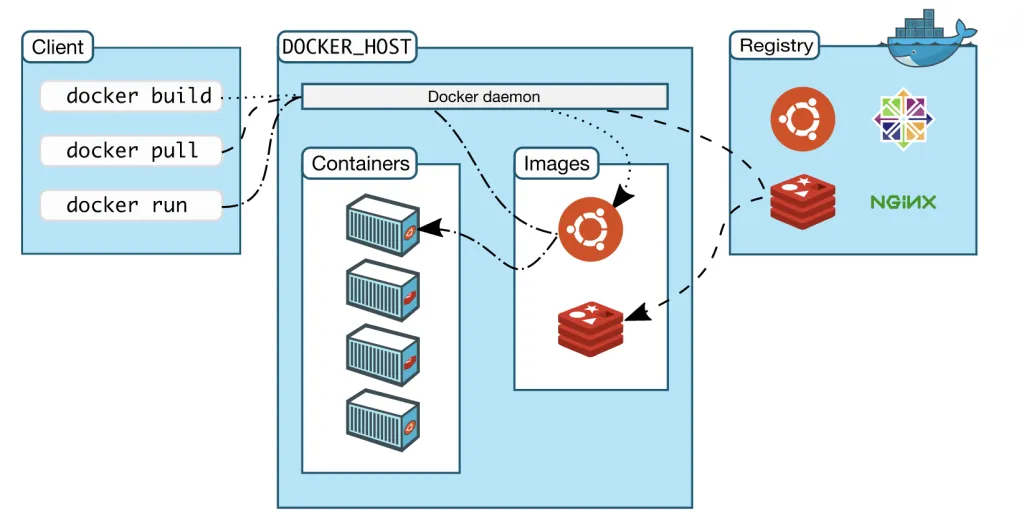
\includegraphics[scale=0.40]{gambar/docker-arch.png}
  % Keterangan gambar yang diinputkan
  \caption{Arsitektur Docker (Sumber: \cite{sysdigteam2024docker})}
  % Label referensi dari gambar yang diinputkan
  \label{fig:Arsitektur Docker}
\end{figure}

% \begin{figure} [H] \centering
%   % Nama dari file gambar yang diinputkan
%   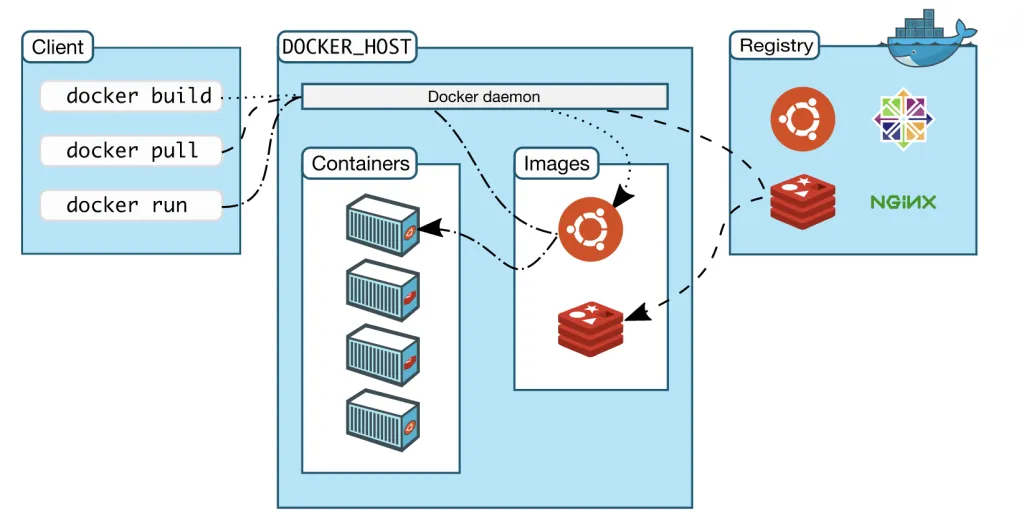
\includegraphics[scale=0.40]{gambar/docker-arch.png}
%   % Keterangan gambar yang diinputkan
%   \caption{Arsitektur Docker (Sumber: \cite{sysdigteam2024docker})}
%   % Label referensi dari gambar yang diinputkan
%   \label{fig:Arsitektur Docker}
% \end{figure}

% \subsection{Kubernetes}

% % \begin{figure} [H] \centering
% %     % Nama dari file gambar yang diinputkan
% %     \includegraphics[scale=0.2]{gambar/Kubernetes_logo_without_workmark.png}
% %     % Keterangan gambar yang diinputkan
% %     \caption{Logo Kubernetes (Sumber: \url{https://kubernetes.io})}
% %     % Label referensi dari gambar yang diinputkan
% %     \label{fig:Kubernetes}
% % \end{figure}

% Kubernetes adalah teknlogi yang sangat populer di dunia \emph{cloud infrastruktur} medern. Sebuah orkestrator \emph{open source} yang berguna untuk melakukan \emph{deployment} aplikasi di dalam kontainer. Awalnya, Kubernetes di kembangkan oleh Google dari pengalaman mereka selama sepuluh tahun lebih. Google men-\emph{deploy} sistem mereka yang andal dan \emph{scalable} di dalam kontainer melalui API yang berorientasi aplikasi.

% Sejak dirilis pada tahun 2014, Kubernetes telah menjadi salah satu teknologi \emph{open soruce} yang paling besar dan paling populer di dunia setelah sistem operasi Linux. Kubernetes API telah menjadi standar industri untuk membangun aplikasi yang bersifat \emph{cloud-native} (mengandalkan kelebihan teknologi \emph{cloud computing} atau komputasi awan), yang tersedia hampir di setiap penyedia layanan \emph{cloud} yang ada.

% Klaster Kubernertes terdiri dari sekumpulan mesin pekerja atau \emph{worker node} yang menjalankan aplikasi dalam kontainer. Setiap klaster paling tidak memiliki satu \emph{worker node}. Node pekerja menempatkan \emph{Pod} yang merupakan komponen beban kerja dari aplikasi. \emph{Control plane} mengelola \emph{node} pekera dan pod dalam \emph{cluster}. Dalam lingkungan produksi pada umumnya, \emph{control plane} dijalankan di beberapa komputer dan klaster menjalankan benyak \emph{node} pekerja untuk memberikan toleransi kesalahan dan ketersedian tinggi(\cite{kuncoro2023kubernetes}).

% Salah satu fitur utama Kubernetes adalah \textit{autoscaling}, yang memungkinkan pengguna untuk menyesuaikan jumlah replika aplikasi secara otomatis berdasarkan kebutuhan sumber daya, seperti penggunaan CPU, memori, atau metrik kustom lainnya. Dengan \textit{autoscaling}, Kubernetes dapat meningkatkan atau mengurangi kapasitas aplikasi secara dinamis, memastikan kinerja aplikasi tetap optimal sekaligus menghemat biaya operasional. Kubernetes juga menyediakan fitur penjadwalan (\textit{scheduling}), yang memungkinkan pengguna untuk mengalokasikan beban kerja ke node tertentu dalam klaster. Penjadwalan ini dapat didasarkan pada berbagai kriteria, seperti ketersediaan sumber daya, label \textit{node}, atau afinitas aplikasi. Selain itu, Kubernetes mendukung penjadwalan tugas secara periodik atau berdasarkan kondisi tertentu, memungkinkan pengguna untuk menjalankan aplikasi sesuai dengan kebutuhan spesifik, seperti tugas batch atau tugas yang dipicu oleh peristiwa tertentu. Selain itu, Kubernetes mendukung \textit{load balancing} dan \textit{service discovery}, yang memungkinkan aplikasi menerima lalu lintas dari pengguna tanpa gangguan, bahkan saat replika aplikasi bertambah atau berkurang (\cite{kubernetesteam2024kubernetes}). 

% Kubernetes secara otomatis mendistribusikan lalu lintas antar replika dan menyediakan mekanisme untuk menemukan layanan lain dalam kluster. Dengan berbagai fitur seperti fault tolerance dan self-healing, Kubernetes memastikan aplikasi tetap berjalan meskipun terjadi kegagalan pada node atau container. Misalnya, Kubernetes dapat secara otomatis memulai ulang container yang gagal, mengganti container yang berhenti, atau memindahkan aplikasi ke node lain yang lebih stabil. Gambar 2.4 merupakan komponen penting yang ada pada Kubernetes.

% \begin{figure} [H] \centering
%     % Nama dari file gambar yang diinputkan
%     \includegraphics[scale=0.4]{gambar/arsitektur-kubernetes.png}
%     % Keterangan gambar yang diinputkan
%     \caption{Arsitektur Kubernetes (Sumber: \cite{kuncoro2023kubernetes}})
%     % Label referensi dari gambar yang diinputkan
%     \label{fig:Arsitektur Kubernetes}
% \end{figure}

% \subsection{K3S}

% K3s adalah distribusi Kubernetes ringan yang dirancang untuk kebutuhan komputasi edge dan lingkungan resource terbatas. K3s dikembangkan oleh Rancher Labs dan menawarkan instalasi yang sederhana, footprint yang kecil, serta kompatibilitas penuh dengan API Kubernetes standar. Dalam penelitian ini, K3s digunakan untuk mengelola orkestrasi \textit{container} Ray Worker dan JupyterHub, mengingat skalabilitas dan kemudahan deployment yang dibutuhkan dalam lingkungan laboratorium yang terbatas sumber dayanya. K3s memungkinkan \textit{deploy} klaster Kubernetes dengan \textit{overhead} minimum dibandingkan dengan Kubernetes penuh, sehingga mempercepat pengembangan dan pengujian sistem 

\newpage



\newpage

\subsection{Penjadwalan GPU dengan Ray}

Penjadwalan GPU merupakan komponen penting dalam sistem komputasi terdistribusi, terutama ketika sumber daya GPU terbatas harus dibagi ke banyak pengguna atau tugas. Ray menyediakan mekanisme penjadwalan tugas berbasis sumber daya yang fleksibel dan dinamis untuk mengelola alokasi GPU secara efisien dalam lingkungan multi-pengguna.

\subsection{JupyterLab}

JupyterLab adalah antarmuka pengguna interaktif berbasis web generasi terbaru dari ekosistem Jupyter yang dirancang untuk mendukung eksplorasi dan analisis data secara komprehensif. Sebagai evolusi dari Jupyter Notebook klasik, JupyterLab menyediakan pengalaman pengembangan yang lebih fleksibel dan extensible dengan arsitektur modular yang mendukung workflow data science modern~\citep{JupyterLabTeam2024}.

\paragraph{Arsitektur JupyterLab}

JupyterLab dibangun dengan arsitektur modular yang terdiri dari beberapa komponen utama:

\textbf{1. Application Shell}\\
Application shell adalah framework utama yang mengelola layout, menu, dan window management. Shell menyediakan:
\begin{itemize}
\item Dockable panels yang dapat disesuaikan
\item Tabbed interface untuk multiple documents
\item Sidebar untuk navigation dan tools
\item Command palette untuk quick access
\item Keyboard shortcuts management
\end{itemize}

\textbf{2. Document Manager}\\
Document manager menangani operasi file dan document lifecycle:
\begin{itemize}
\item File browser dengan real-time synchronization
\item Document registry untuk berbagai file types
\item Auto-save dan version control integration
\item Context menu dengan action-specific options
\end{itemize}

\textbf{3. Kernel Management System}\\
JupyterLab menggunakan kernel-based architecture untuk eksekusi kode:
\begin{itemize}
\item Multi-kernel support (Python, R, Julia, Scala, dll)
\item Kernel lifecycle management (start, stop, restart, interrupt)
\item Session management untuk multiple notebooks
\item Real-time kernel status monitoring
\item Resource usage tracking per kernel
\end{itemize}

\begin{lstlisting}[language=Python]
# Contoh interaksi dengan kernel
import psutil
import GPUtil

# Monitor system resources
cpu_usage = psutil.cpu_percent()
memory_usage = psutil.virtual_memory().percent

# Check GPU availability
gpus = GPUtil.getGPUs()
for gpu in gpus:
    print(f"GPU {gpu.id}: {gpu.name}, Memory: {gpu.memoryUsed}/{gpu.memoryTotal}MB")
\end{lstlisting}

\paragraph{Extension System dan Plugin Architecture}

JupyterLab memiliki sistem ekstensi yang powerful untuk customization:

\textbf{Extension Types:}
\begin{itemize}
\item \textbf{Frontend Extensions}: Menambahkan UI components dan functionality
\item \textbf{Server Extensions}: Memperluas server-side capabilities
\item \textbf{Kernel Extensions}: Menambahkan kernel-specific features
\item \textbf{Theme Extensions}: Customization visual appearance
\end{itemize}

\textbf{Plugin Ecosystem:}
\begin{itemize}
\item \texttt{jupyterlab-git}: Git integration untuk version control
\item \texttt{jupyterlab-variableInspector}: Variable debugging tools
\item \texttt{jupyterlab-system-monitor}: Real-time resource monitoring
\item \texttt{jupyterlab-nvidia-smi}: GPU monitoring dan management
\item \texttt{jupyterlab-tensorboard}: TensorBoard integration
\end{itemize}

\paragraph{Multi-Document Interface}

JupyterLab menyediakan integrated development environment dengan dukungan multiple document types:

\begin{itemize}
\item \textbf{Notebooks}: Interactive computing dengan cells untuk code, markdown, dan output
\item \textbf{Code Editor}: Syntax highlighting dan IntelliSense untuk berbagai bahasa
\item \textbf{Terminal}: Integrated terminal dengan full shell access
\item \textbf{File Viewer}: Preview untuk images, JSON, CSV, dan file types lainnya
\item \textbf{Data Viewer}: Tabular data exploration dengan sorting dan filtering
\end{itemize}

\paragraph{Collaborative Features}

JupyterLab mendukung real-time collaboration:
\begin{itemize}
\item \textbf{Real-time Document Sharing}: Multiple users dapat edit notebook simultaneously
\item \textbf{Comment System}: Annotation dan discussion dalam notebooks
\item \textbf{Version Control}: Git integration untuk collaborative development
\item \textbf{Workspace Sharing}: Export/import workspace configurations
\end{itemize}

\paragraph{Kontainerisasi dengan Docker}

JupyterLab dapat dijalankan dalam Docker container untuk isolated environments:

\textbf{Container Benefits:}
\begin{itemize}
\item \textbf{Environment Isolation}: Setiap user mendapat environment terpisah
\item \textbf{Dependency Management}: Pre-configured libraries dan tools
\item \textbf{Scalability}: Easy deployment dan horizontal scaling
\item \textbf{Security}: Sandboxed execution environment
\end{itemize}

\textbf{Docker Configuration Example:}
\begin{lstlisting}[language=bash]
# Dockerfile untuk JupyterLab dengan GPU support
FROM jupyter/tensorflow-notebook:latest

# Install additional packages
RUN pip install jupyterlab-nvidia-smi \
                jupyterlab-system-monitor \
                ray[default] \
                torch torchvision

# Configure JupyterLab
RUN jupyter lab build

# Mount volumes untuk persistent storage
VOLUME ["/home/jovyan/work"]

# Expose JupyterLab port
EXPOSE 8888

# GPU runtime support
ENV NVIDIA_VISIBLE_DEVICES all
ENV NVIDIA_DRIVER_CAPABILITIES compute,utility
\end{lstlisting}

\paragraph{GPU Computing Support}

JupyterLab menyediakan dukungan komprehensif untuk GPU computing:

\textbf{CUDA Integration:}
\begin{itemize}
\item Automatic CUDA device detection
\item \texttt{CUDA\_VISIBLE\_DEVICES} environment variable management
\item GPU memory monitoring dan profiling tools
\item NVIDIA System Management Interface (nvidia-smi) integration
\end{itemize}

\textbf{Deep Learning Framework Support:}
\begin{itemize}
\item \textbf{PyTorch}: Native CUDA support dengan automatic device placement
\item \textbf{TensorFlow}: GPU acceleration dengan XLA compilation
\item \textbf{JAX}: Hardware-accelerated computing dengan GPU/TPU support
\item \textbf{CuPy}: NumPy-compatible library untuk GPU computing
\end{itemize}

\begin{lstlisting}[language=Python]
# Contoh GPU usage dalam JupyterLab
import torch
import tensorflow as tf

# Check GPU availability
print(f"PyTorch CUDA available: {torch.cuda.is_available()}")
print(f"TensorFlow GPU devices: {tf.config.list_physical_devices('GPU')}")

# Monitor GPU memory
if torch.cuda.is_available():
    gpu_memory = torch.cuda.get_device_properties(0).total_memory
    gpu_memory_used = torch.cuda.memory_allocated(0)
    print(f"GPU Memory: {gpu_memory_used/1e9:.2f}GB / {gpu_memory/1e9:.2f}GB")
\end{lstlisting}

\paragraph{Resource Monitoring dan Management}

JupyterLab dapat diintegrasikan dengan monitoring tools untuk real-time resource tracking:

\begin{itemize}
\item \textbf{System Metrics}: CPU, RAM, disk usage monitoring
\item \textbf{GPU Metrics}: GPU utilization, memory usage, temperature
\item \textbf{Process Monitoring}: Kernel resource consumption tracking
\item \textbf{Custom Dashboards}: Extensible monitoring dengan custom widgets
\end{itemize}

\paragraph{Security Features}

JupyterLab menyediakan berbagai security features untuk multi-user environments:

\begin{itemize}
\item \textbf{Authentication}: Token-based authentication dengan configurable timeout
\item \textbf{HTTPS Support}: TLS encryption untuk secure communication
\item \textbf{Content Security Policy}: Protection against XSS attacks
\item \textbf{Sandboxing}: Process isolation dalam container environments
\item \textbf{Access Control}: File system permissions dan user workspace isolation
\end{itemize}

\paragraph{Performance Optimization}

JupyterLab dapat dioptimasi untuk performance dalam production environments:

\begin{itemize}
\item \textbf{Kernel Culling}: Automatic cleanup idle kernels untuk resource efficiency
\item \textbf{Memory Management}: Configurable memory limits per user session
\item \textbf{Caching}: Browser caching untuk faster loading
\item \textbf{Lazy Loading}: On-demand loading untuk large notebooks
\item \textbf{Resource Limits}: CPU dan memory quotas per container
\end{itemize}

\paragraph{Integration dengan Ray Framework}

Dalam konteks distributed computing, JupyterLab dapat diintegrasikan dengan Ray:

\begin{lstlisting}[language=Python]
import ray
import time

# Initialize Ray cluster connection
ray.init(address='ray://head-node:10001')

# Distributed computing example
@ray.remote(num_gpus=1)
def gpu_compute_task(data):
    # GPU-accelerated computation
    import torch
    device = torch.device('cuda')
    tensor = torch.tensor(data).to(device)
    result = torch.matmul(tensor, tensor.T)
    return result.cpu().numpy()

# Submit tasks to Ray cluster
futures = [gpu_compute_task.remote(data) for data in dataset]
results = ray.get(futures)
\end{lstlisting}

\paragraph{Relevansi dengan Tugas Akhir}

Dalam konteks tugas akhir "Pengelolaan Penggunaan Infrastruktur GPU untuk Pengguna Berbasis Docker Container Menggunakan JupyterLab", JupyterLab berperan sebagai:

\begin{itemize}
\item \textbf{User Interface Layer}: Menyediakan web-based interface untuk akses GPU resources
\item \textbf{Development Environment}: Integrated environment untuk GPU computing dan ML development
\item \textbf{Resource Visualization}: Real-time monitoring GPU usage dan cluster status
\item \textbf{Collaboration Platform}: Multi-user workspace untuk shared research projects
\item \textbf{Integration Hub}: Central point untuk connecting dengan Ray distributed computing
\item \textbf{Container Runtime}: Standardized environment untuk reproducible computing
\end{itemize}

Dengan fitur-fitur komprehensif ini, JupyterLab menjadi foundation yang ideal untuk membangun sistem pengelolaan GPU terdistribusi yang user-friendly, scalable, dan efficient dalam lingkungan multi-pengguna.


\subsection{JupyterHub}

JupyterHub adalah platform open-source yang memungkinkan banyak pengguna untuk mengakses dan menjalankan lingkungan Jupyter Notebook secara terisolasi melalui antarmuka web. Dirancang untuk mendukung skenario multi-pengguna, JupyterHub sangat cocok digunakan dalam lingkungan pendidikan, penelitian, dan industri yang memerlukan akses bersama ke sumber daya komputasi.

\paragraph{Arsitektur Utama JupyterHub}\mbox{}\\
JupyterHub terdiri dari tiga komponen utama yang bekerja secara sinergis:


\begin{enumerate}
\item \textbf{Hub:} Komponen inti yang bertanggung jawab atas manajemen akun pengguna, proses autentikasi, dan koordinasi peluncuran server notebook individu melalui mekanisme yang disebut Spawner.
\item \textbf{Proxy:} Berfungsi sebagai gerbang utama yang menerima semua permintaan HTTP dari pengguna dan meneruskannya ke Hub atau server notebook pengguna yang sesuai. Secara default, JupyterHub menggunakan configurable-http-proxy yang dibangun di atas node-http-proxy.
\item \textbf{Single-User Notebook:} Server Jupyter Notebook yang dijalankan secara terpisah untuk setiap pengguna setelah proses autentikasi berhasil. Server ini memungkinkan pengguna untuk menjalankan kode dan berinteraksi dengan lingkungan Jupyter secara pribadi.
\end{enumerate}

\paragraph{Alur Kerja JupyterHub}\mbox{}\\
Proses interaksi pengguna dengan JupyterHub dapat dijelaskan sebagai berikut:

\begin{enumerate}
\item {Akses Awal:} Pengguna mengakses JupyterHub melalui browser web dengan mengunjungi alamat IP atau nama domain yang telah dikonfigurasi.
\item {Autentikasi:} Data login yang dimasukkan oleh pengguna dikirim ke komponen Authenticator untuk validasi. Jika valid, pengguna akan dikenali dan diizinkan untuk melanjutkan.
\item {Peluncuran Server Notebook:} Setelah autentikasi berhasil, JupyterHub akan meluncurkan instance server notebook khusus untuk pengguna tersebut menggunakan Spawner.
\item {Konfigurasi Proxy:} Proxy dikonfigurasi untuk meneruskan permintaan dengan URL tertentu (misalnya, \textbf{/user/[username]}) ke server notebook pengguna yang sesuai.
\item {Penggunaan Lingkungan Jupyter:} Pengguna diarahkan ke server notebook pribadi mereka, di mana mereka dapat mulai bekerja dengan lingkungan Jupyter seperti biasa.
\end{enumerate}

\paragraph{Melakukan kustomisasi dan menambah extension}\mbox{}\\
JupyterHub dirancang dengan fleksibilitas tinggi, memungkinkan kustomisasi melalui dua komponen utama:

\begin{itemize}
  \item \textbf{Authenticator:} Mengelola proses autentikasi pengguna. JupyterHub mendukung berbagai metode autentikasi, termasuk PAM (Pluggable Authentication Modules), OAuth, LDAP, dan lainnya.
  
  \item \textbf{Spawner:} Mengontrol cara peluncuran server notebook untuk setiap pengguna. Beberapa jenis Spawner yang umum digunakan antara lain:
  \begin{itemize}
    \item \textbf{LocalProcessSpawner:} Meluncurkan server notebook sebagai proses lokal di mesin yang sama.
    \item \textbf{DockerSpawner:} Menjalankan server notebook dalam container Docker, memberikan isolasi lingkungan yang lebih baik.
    \item \textbf{KubeSpawner:} Menggunakan Kubernetes untuk mengelola dan menskalakan server notebook di lingkungan klaster.
  \end{itemize}
\end{itemize}

Kemampuan untuk menyesuaikan dan memperluas JupyterHub melalui Authenticator dan Spawner memungkinkan integrasi yang mulus dengan berbagai infrastruktur dan kebutuhan spesifik pengguna.

\subsection{Ray Framework}

Ray merupakan sebuah \textit{framework} \textit{open-source} yang dirancang untuk membangun dan menjalankan aplikasi komputasi paralel dan terdistribusi secara efisien. Framework ini menyediakan abstraksi tingkat tinggi yang memungkinkan pengembang untuk membuat aplikasi yang skalabel dan mudah dijalankan pada klaster komputasi yang terdiri dari banyak node (\cite{moritz2018ray}).

Ray mendukung dua paradigma pemrograman utama:

\textbf{1. Task-based Computing (Stateless)}\\
Task-based computing memungkinkan pengguna untuk menjalankan fungsi Python secara paralel menggunakan dekorator \texttt{@ray.remote}. Model ini bersifat stateless dan cocok digunakan untuk proses komputasi yang dapat dibagi menjadi unit-unit kecil independen.

\textbf{2. Actor-based Computing (Stateful)}\\
Paradigma ini memungkinkan pengguna untuk membuat komponen yang mempertahankan state selama siklus hidupnya. Cocok untuk aplikasi dengan shared state atau layanan yang berjalan terus-menerus.

\paragraph{Arsitektur Ray}\mbox{}\\
Arsitektur Ray terbagi menjadi dua lapisan utama, yaitu \textbf{Application Layer} dan \textbf{System Layer (Backend)}.

\paragraph{Application Layer}\mbox{}\\
Pada lapisan aplikasi, terdapat beberapa komponen utama:

\begin{itemize}
\item \textbf{Driver}: Komponen yang memulai eksekusi program Ray dan bertanggung jawab dalam mengatur tasks dan actors.
\item \textbf{Worker}: Unit eksekusi stateless yang digunakan untuk menjalankan fungsi-fungsi remote.
\item \textbf{Actor}: Unit eksekusi stateful yang mempertahankan data selama proses berjalan.
\end{itemize}

\paragraph{System Layer (Backend)}\mbox{}\\
Lapisan sistem ini mencakup manajemen koordinasi, scheduling, dan penyimpanan objek:

\textbf{1. Object Store}\
Object Store adalah penyimpanan berbasis memori untuk menyimpan objek hasil eksekusi:
\begin{itemize}
\item Mendukung \textit{zero-copy} antar proses
\item Manajemen memori otomatis
\item Penyimpanan efisien untuk objek besar
\end{itemize}

\textbf{2. Raylet (Local Scheduler + Object Manager)}\
\begin{itemize}
\item Menangani penjadwalan tasks lokal
\item Mengelola transfer objek antar node
\item Berinteraksi dengan Global Control Store (GCS)
\end{itemize}

\textbf{3. Global Control Store (GCS)}\
Komponen pusat metadata dan koordinasi antar node:
\begin{itemize}
\item Menyimpan metadata objek, status tasks, actors, dan nodes
\item Menyediakan event logs untuk debugging
\end{itemize}

\textbf{4. Global Scheduler}\
Mengatur penjadwalan global saat node lokal tidak memiliki resource yang mencukupi.

\begin{figure} [H] \centering
  % Nama dari file gambar yang diinputkan
  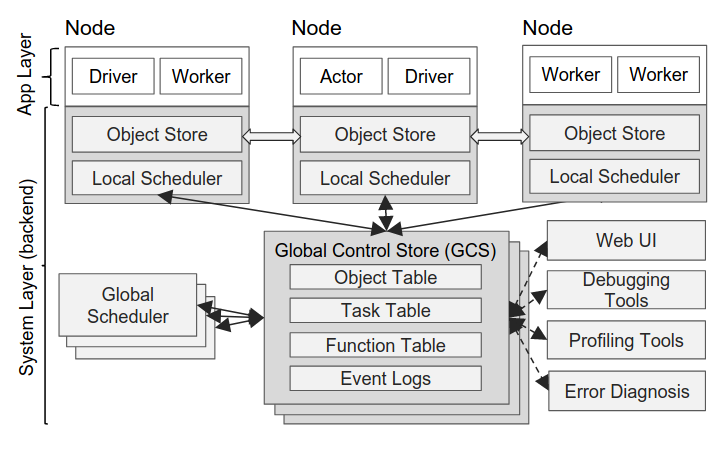
\includegraphics[scale=0.5]{gambar/arsitektur-ray.png}
  % Keterangan gambar yang diinputkan
  \caption{Komponen \emph{RAY} (Sumber: \cite{moritz2018ray})}
  % Label referensi dari gambar yang diinputkan
  \label{fig:Arsitekur RAY}
\end{figure}

\paragraph{Konsep Resource dalam Ray}

Ray mendefinisikan resource sebagai pasangan key-value dimana key menunjukkan nama resource dan value adalah kuantitas float~\citep{RayResources2024}. Ray memiliki dukungan native untuk CPU, GPU, dan memory resource types yang disebut sebagai pre-defined resources. Selain itu, Ray juga mendukung custom resources untuk kebutuhan spesifik.

Resource dalam Ray bersifat logical dan tidak harus memiliki mapping 1-to-1 dengan resource fisik. Secara default, logical resources dikonfigurasi berdasarkan aturan berikut:
\begin{itemize}
\item \textbf{Number of logical CPUs (\texttt{num\_cpus})}: Diset sesuai jumlah CPU fisik pada mesin/container
\item \textbf{Number of logical GPUs (\texttt{num\_gpus})}: Diset sesuai jumlah GPU fisik pada mesin/container
\item \textbf{Memory}: Diset sebesar 70\% dari available memory ketika Ray runtime dimulai
\end{itemize}

\paragraph{Mekanisme Penjadwalan Ray}

Ray menggunakan strategi penjadwalan hierarkis yang terdiri dari Global Scheduler dan Local Scheduler. Untuk setiap task atau actor, Ray akan memilih node berdasarkan faktor-faktor berikut~\parencite{RayScheduling2024}:

\textbf{Status Node:}
\begin{enumerate}
\item \textbf{Feasible}: Node memiliki resource yang diperlukan untuk menjalankan task atau actor
   \begin{itemize}
   \item \textit{Available}: Node memiliki resource yang diperlukan dan sedang tersedia
   \item \textit{Unavailable}: Node memiliki resource yang diperlukan tetapi sedang digunakan
   \end{itemize}
\item \textbf{Infeasible}: Node tidak memiliki resource yang diperlukan (contoh: CPU-only node tidak feasible untuk GPU task)
\end{enumerate}

\textbf{Algoritma Penjadwalan:}
Ray menjadwalkan tasks atau actors ke grup top-k nodes. Node-node diurutkan berdasarkan prioritas:
\begin{enumerate}
\item Mengutamakan node yang sudah memiliki tasks atau actors terjadwal (untuk locality)
\item Mengutamakan node dengan resource utilization rendah (untuk load balancing)
\item Dalam grup top-k, node dipilih secara random untuk meningkatkan load-balancing
\end{enumerate}

Nilai k dihitung sebagai maksimum dari:
\begin{itemize}
\item (jumlah node dalam cluster × \texttt{RAY\_scheduler\_top\_k\_fraction})
\item \texttt{RAY\_scheduler\_top\_k\_absolute}
\end{itemize}
Secara default, nilai ini adalah 20\% dari total jumlah node.

\paragraph{GPU Resource Requirements}

Ray memungkinkan spesifikasi resource requirements untuk tasks atau actors melalui decorator \texttt{ray.remote()}. Untuk GPU, persyaratan resource yang lebih besar dari 1 harus berupa bilangan bulat. Contoh:

\begin{lstlisting}[language=Python]
# Task yang membutuhkan 1 GPU
@ray.remote(num_gpus=1)
def gpu_task():
    return "Hello from GPU"

# Actor yang membutuhkan 2 GPU
@ray.remote(num_gpus=2)
class GPUActor:
    def __init__(self):
        self.device = torch.cuda.current_device()
\end{lstlisting}

\paragraph{GPU Isolation dan Visibility}

Ray menyediakan GPU isolation dalam bentuk visible devices dengan secara otomatis mengatur environment variable \texttt{CUDA\_VISIBLE\_DEVICES}. Sebagian besar ML frameworks akan menghormati pengaturan ini untuk tujuan GPU assignment~\citep{RayResources2024}.

Penting untuk dicatat bahwa resource requirements tidak memberlakukan batasan pada penggunaan resource fisik aktual. Ray tidak mencegah task \texttt{num\_gpus=1} menggunakan beberapa GPU fisik jika tersedia. Menjadi tanggung jawab pengguna untuk memastikan tasks atau actors tidak menggunakan lebih banyak resource dari yang dispesifikasikan.

\paragraph{Custom Resources untuk GPU Management}

Ray memungkinkan penggunaan custom resources sebagai label untuk menandai nodes dan mencapai label-based affinity scheduling~\citep{RayCustomResources2019}. Contoh penggunaan:

\begin{lstlisting}[language=Python]
# Menggunakan custom resource sebagai label
@ray.remote(resources={"gpu_type_v100": 0.001})
def specialized_gpu_task():
    return "Running on V100 GPU"

# Menginisialisasi Ray dengan custom resources
ray.init(resources={"gpu_type_v100": 4, "gpu_type_a100": 2})
\end{lstlisting}

\paragraph{Fractional GPU Allocation}

Ray mendukung alokasi fractional GPU, memungkinkan multiple workers untuk berbagi CUDA device yang sama. Hal ini berguna untuk memaksimalkan utilization GPU ketika individual tasks tidak memerlukan seluruh GPU:

\begin{lstlisting}[language=Python]
# Task dengan 0.5 GPU
@ray.remote(num_gpus=0.5)
def fractional_gpu_task():
    return "Sharing GPU resources"
\end{lstlisting}

\paragraph{Advanced Scheduling Strategies}

Ray menyediakan beberapa scheduling strategies untuk kontrol yang lebih fine-grained:

\begin{enumerate}
\item \textbf{NodeAffinitySchedulingStrategy}: Memungkinkan task atau actor dijadwalkan ke node spesifik berdasarkan node ID
\item \textbf{PlacementGroupSchedulingStrategy}: Memungkinkan bundling tasks dan actors dengan resource requirements yang terkait
\item \textbf{Default Strategy}: Menggunakan algoritma penjadwalan standar Ray
\end{enumerate}

\paragraph{Memory-Aware Scheduling}

Ray juga mendukung memory-aware scheduling dengan memungkinkan spesifikasi memory requirements:

\begin{lstlisting}[language=Python]
# Task dengan GPU dan memory requirements
@ray.remote(num_gpus=1, memory=2*1024*1024*1024)  # 2GB memory
def gpu_memory_task():
    return "GPU task with memory requirements"
\end{lstlisting}

\paragraph{Integration dengan Container dan JupyterHub}

Dalam konteks tugas akhir ini, penjadwalan GPU Ray terintegrasi dengan:
\begin{itemize}
\item \textbf{Docker Container}: Setiap container JupyterLab dapat menjadi Ray worker dengan akses GPU yang terisolasi
\item \textbf{JupyterHub Spawner}: Custom spawner dapat menggunakan informasi dari discovery service untuk memilih node dengan GPU available
\item \textbf{Multi-Node Cluster}: Ray cluster dapat spawn multiple physical machines dengan GPU resources yang terdistribusi
\end{itemize}

Dengan mekanisme penjadwalan yang komprehensif ini, Ray mampu mengelola alokasi GPU secara efisien dalam lingkungan multi-pengguna, memastikan resource utilization yang optimal sambil mempertahankan fairness dan isolation antar pengguna.
\cleardoublepage

% Bab 3 desain dan implementasi
\chapter{DESAIN DAN IMPLEMENTASI}
\label{chap:desainimplementasi}

% Ubah bagian-bagian berikut dengan isi dari desain dan implementasi

Penelitian ini dilaksanakan sesuai \lipsum[1][1-5]

\section{Deskripsi Sistem}
\label{sec:deskripsisistem}

Sistem akan dibuat dengan \lipsum[1-2]

\section{Implementasi Alat
  \label{sec:implementasi alat}}

Alat diimplementasikan dengan \lipsum[1]

% Contoh pembuatan potongan kode
\begin{lstlisting}[
  language=C++,
  caption={Program halo dunia.},
  label={lst:halodunia}
]
#include <iostream>

int main() {
    std::cout << "Halo Dunia!";
    return 0;
}
\end{lstlisting}

\lipsum[2-3]

% Contoh input potongan kode dari file
\lstinputlisting[
  language=Python,
  caption={Program perhitungan bilangan prima.},
  label={lst:bilanganprima}
]{program/bilangan-prima.py}

\lipsum[4]

\cleardoublepage

% Bab 4 pengujian dan analisis
\chapter{PENGUJIAN DAN ANALISIS}
\label{chap:pengujiananalisis}

% Ubah bagian-bagian berikut dengan isi dari pengujian dan analisis

Pada penelitian ini dipaparkan \lipsum[1][1-5]

\section{Skenario Pengujian}
\label{sec:skenariopengujian}

Pengujian dilakukan dengan \lipsum[1-2]

\section{Evaluasi Pengujian}
\label{sec:analisispengujian}

Dari pengujian yang \lipsum[1]

% Contoh pembuatan tabel
\begin{longtable}{|c|c|c|}
  \caption{Hasil Pengukuran Energi dan Kecepatan}
  \label{tb:EnergiKecepatan}                                   \\
  \hline
  \rowcolor[HTML]{C0C0C0}
  \textbf{Energi} & \textbf{Jarak Tempuh} & \textbf{Kecepatan} \\
  \hline
  10 J            & 1000 M                & 200 M/s            \\
  20 J            & 2000 M                & 400 M/s            \\
  30 J            & 4000 M                & 800 M/s            \\
  40 J            & 8000 M                & 1600 M/s           \\
  \hline
\end{longtable}

\lipsum[2-4]

\cleardoublepage

% Bab 5 penutup
\chapter{PENUTUP}
\label{chap:penutup}

% Ubah bagian-bagian berikut dengan isi dari penutup

\section{Kesimpulan}
\label{sec:kesimpulan}

Berdasarkan hasil pengujian yang \lipsum[1][1-3] sebagai berikut:

\begin{enumerate}[nolistsep]

  \item Pembuatan \lipsum[2][1-3]

  \item \lipsum[2][4-6]

  \item \lipsum[2][7-10]

\end{enumerate}

\section{Saran}
\label{chap:saran}

Untuk pengembangan lebih lanjut pada \lipsum[1][1-3] antara lain:

\begin{enumerate}[nolistsep]

  \item Memperbaiki \lipsum[2][1-3]

  \item \lipsum[2][4-6]

  \item \lipsum[2][7-10]

\end{enumerate}

\cleardoublepage

\chapter*{DAFTAR PUSTAKA}
\addcontentsline{toc}{chapter}{DAFTAR PUSTAKA}
\renewcommand\refname{}
\vspace{2ex}
\renewcommand{\bibname}{}
\begingroup
\def\chapter*#1{}
\printbibliography
\endgroup
\cleardoublepage

% Biografi penulis
\begin{center}
  \Large
  \textbf{BIOGRAFI PENULIS}
\end{center}

\addcontentsline{toc}{chapter}{BIOGRAFI PENULIS}

\vspace{2ex}

\begin{wrapfigure}{L}{0.3\textwidth}
  \centering
  \vspace{-3ex}
  % Ubah file gambar berikut dengan file foto dari mahasiswa
  
\includegraphics[width=0.3\textwidth]{gambar/elon.jpg}
  \vspace{-4ex}
\end{wrapfigure}

% Ubah kalimat berikut dengan biografi dari mahasiswa
\name{}, lahir pada \lipsum[1]

\lipsum[2]

\cleardoublepage

\end{document}
